% Template Tesis Pregrado/Postgrado de la Facultad de
% Ingenieria de la Universidad de Santiago de Chile

% Autor: Alfonso Suárez Cornejo

%-----------------------------------------------------------------------------------------------------------------------------------------

% IMPORTACIÓN DE PAQUETES

% Clase de documento, formato libro.
\documentclass[a4paper,10pt,openany,oneside]{book}
% Documento configurado para imprimir a una cara (oneside), para cambiar a impresión por 2 caras modificar a "twoside".

% Paquete para el soporte de idiomas.
\usepackage[spanish,es-tabla]{babel}
\usepackage[utf8]{inputenc}

% Paquete para la manipulación de imágenes.
\usepackage{graphicx}

% Paquete para la referencias links y marcadores en el menu del pdf
\usepackage[bookmarksnumbered,bookmarksopen=false]{hyperref}

% Paquete para agregar "custom" bookmarks
\usepackage{bookmark}

% Márgenes de la hoja
\usepackage[a4paper,top=2.5cm,bottom=2.5cm,left=4cm,right=2.5cm]{geometry}
\newgeometry{top=2.5cm,bottom=2.5cm,left=4cm,right=2.5cm}

% Paquete para encabezados o pies de página.
\usepackage{fancyhdr}

% Paquete para la prevensión de aparición 
% de pies de página, encabezados y numeración.
\usepackage{emptypage}

% Paquete para la adecuación de cuadros y tablas.
\usepackage{float}

% Paquete que permite la construcción de tablas
% que abarquen mas de una página.
\usepackage{longtable}

% Paquete para mejorar la compatibilidad en la manipulación de comillas y citas en diferentes idiomas (biblatex)
\usepackage{csquotes}

% Paquete que ofrece el soporte de citación estilo APA.
\usepackage[style=apa, backend=biber, maxcitenames=3, maxbibnames=10, maxnames=10, minnames=3]{biblatex}
\addbibresource{referencias.bib}
% El argumento 'maxcitenames' nos permite indicar el número maximo de autores en texto, es decir, que si la referencia tiene 4 o más autores aparecera et al.
% El argumento 'maxbibnames' nos permite indicar el número maximo de autores en "REFERENCIAS BIBLIOGRAFICAS", En APA 7ma edición se deben escribir todos los autores, por lo que para evitar que no ocurra tiene valor de 10 (en caso de tener referencias de más autores, aumentar el valor).

% Paquetes para el uso de fórmulas matemáticas.
\usepackage{amsmath, amsthm, amssymb}

% Paquete para la inclusión de Anexos
\usepackage{appendix}

% Paquete para la graficación
\usepackage{tikz}
\usetikzlibrary{shapes,arrows}

% Paquete para el espaciado automático entre párrafos
% ya no es necesario el "//"
\usepackage{parskip}

% Paquete para espaciar el titulo de las tablas 
\usepackage{caption}
\usepackage{subcaption}

% Paquete para eliminar los espacios en blanco 
% entre titulos/subtitulos/etc.
\usepackage[compact]{titlesec}

% Paquete pora importar de forma anidada
\usepackage{import}

% Paquete que simplifica la notación de unidades físicas medidas etc 
\usepackage{siunitx}

% Paquete para la configuración de listas
\usepackage{enumitem}

% Paquete para modificar el comportamiento de los listings
\usepackage{listings}

% Paquete para el manejo de colores
\usepackage{xcolor}

% Llamamos nuestro paquete "docstyle" de la carpeta config
\usepackage{config/docstyle}

% Paquete que nos ayuda a evitar los cortes de palabras
\usepackage[none]{hyphenat}

% Paquete para controlar el interlineado del documento
\usepackage{setspace}

% Declaramos nuestro propio caption (titulo tablas y figuras)
\DeclareCaptionFormat{custom}{\textit{\small#1#2}\textit{\small#3}}

% Paquete para el estilo de letra Helvetica (reemplazo de arial)
\usepackage{helvet}

% Paquete que permite modificar el formato de titulo de capítulos, secciones y subsecciones.
% Probamos este
\usepackage{titletoc}
\usepackage{titlesec}

% Quitamos la numeración de las secciones. 
\setcounter{secnumdepth}{0}
% Aseguramos que aparecerán las subsubsecciones en la tabla de contenidos
\setcounter{tocdepth}{3}

% Configuración de la bibliografia para establecer el 'Recuperado de' los enlaces en las referencias bibliograficas. 
\DeclareFieldFormat{url}{\bibstring{retrieved}\addspace\bibstring{from}\space\url{#1}}
\DeclareFieldFormat{doi}{\bibstring{retrieved}\addspace\bibstring{from}\space\url{https://doi.org/#1}}
\DefineBibliographyStrings{spanish}{
  retrieved = {Recuperado},
  from = {de}
}

%-----------------------------------------------------------------------------------------------------------------------------------------

% CUERPO TESIS

\raggedbottom\begin{document}
    % RENOMBRANDO

% Indices renombrados
% Renombrnado el indice general a 'TABLA DE CONTENIDOS'
\renewcommand{\contentsname}{\hfill\large TABLA DE CONTENIDOS\hfill}
% Ajustando el espaciado vertical (despes del titulo)
\makeatletter
\patchcmd{\tableofcontents}{\@starttoc}{\vspace{-10pt}\@starttoc}{}{}
\makeatother

% Renombrando el indice de figuras 
\renewcommand{\listfigurename}{\hfill\large INDICE DE FIGURAS\hfill}
% Ajustando el espaciado vertical (despues del titulo)
%\makeatletter
%\patchcmd{\listoffigures}{\@starttoc}%{\vspace{0pt}\@starttoc}{}{}
%\makeatother

% Renombrando el indice de tablas
\renewcommand{\listtablename}{\hfill\large INDICE DE TABLAS\hfill}
% Ajustando el espaciado vertical (despues del titulo)
%\makeatletter
%\patchcmd{\listoftables}{\@starttoc}{\vspace{0pt}\@starttoc}{}{}
%\makeatother

% Renombrando la bibliografía
\renewcommand{\bibname}{\large REFERENCIAS BIBLIOGRAFICAS}
%------------------------------------------------------------------
% Estableciendo terminaciones de las referencias bibliograficas
%\renewcommand{\BOthers}[1]{et al.\hbox{}}
%\renewcommand{\BAvailFrom}[1]{Recuperado de\hbox{}}
%\renewcommand{\BRetrievedFrom}[1]{Recuperado de }
%\renewcommand{\BRetrieved}[1]{}
%------------------------------------------------------------------

% Configurando el tamaño de titulos de capítulos y subcapítulos
\titleformat*{\section}{\large\bfseries}
\titleformat*{\subsection}{\large\bfseries}
\titleformat*{\subsubsection}{\large\bfseries}
\titleformat{name=\chapter}[display]{\large\bfseries}{\thechapter}{10pt}{\large}
% Ajustando el espacio vertical superior (-20pt) y el espacio vertical inferior (-15pt) de los capítulos
\titlespacing*{\chapter}{0pt}{-20pt}{15pt}


% Creamos contadores para los capítulos
\newcounter{cap1}
\newcounter{cap2}
\newcounter{cap3}
\newcounter{cap4}
\newcounter{cap5}
\newcounter{cap6}
% Creamos los contadores para las figuras y tablas
\newcounter{figura}
\newcounter{tabla}

% Inicializamos los contadores con su valor respectivo
% Capitulos
\setcounter{cap1}{1}
\setcounter{cap2}{2}
\setcounter{cap3}{3}
\setcounter{cap4}{4}
\setcounter{cap5}{5}
\setcounter{cap6}{6}
% Figuras y Tablas
\setcounter{figura}{1}
\setcounter{tabla}{1}

% Configurando caption (titulo figuras y tablas)
\captionsetup{format=custom}

% Configurando el espaciado entre "itemize/enumerate items"
\setlist[itemize]{noitemsep, topsep=3mm}
\setlist[enumerate]{noitemsep, topsep=3mm}

% Espacios entre autores en "Bibliografia"
%\let\OLDthebibliography\thebibliography
%\renewcommand\thebibliography[1]{
%  \OLDthebibliography{#1}
%  \setlength{\parskip}{3mm}
%  \setlength{\itemsep}{3mm plus 0.3ex}
%}

    %\newgeometry{top=2.5cm,bottom=2.5cm,left=4cm,right=2.5cm}
\begin{titlepage}
%\hfill
    \begin{minipage}{12cm}
        \begin{center}
            \textbf{\Large\MakeUppercase{\nombreUniversidad}}\\
            \textbf{\Large\MakeUppercase{\nombreFacultad}}\\
            \textbf{\Large\nombreCarrera}
        \end{center}
    \end{minipage}
    %\hfill
    \begin{minipage}{2cm}
        \begin{center}
            
\includegraphics[width=2cm,height=2.55cm]{logo_usach.jpg}
        \end{center}
    \end{minipage}
    \vspace{2.5cm}\\

    \begin{center}
        \textbf{\Large\MakeUppercase{\nombreProyecto}}
    \end{center}
    \vspace{1cm}
    
    \begin{center}
        \textbf{\normalsize\MakeUppercase{\nombreAutorUno}}\\
        \textbf{\normalsize\MakeUppercase{\nombreAutorDos}}
    \end{center}
    \vspace{3.5cm}
    
    \raggedleft\begin{minipage}{5cm}
        \textbf{\normalsize\MakeUppercase\nombreTutor}\\
        \\
        \textbf{\normalsize\MakeUppercase\grado}\\
    \end{minipage}
    \vspace{3.2cm}
    
    \centering\textnormal{\MakeUppercase{\textbf{\nombreCiudadPais}}}\\
    \centering\textnormal{\textbf{\fecha}}

\end{titlepage}
%\restoregeometry
    %vspace{-40pt}
    \frontmatter\pagenumbering{roman}
        \chapter*{\begin{center}RESUMEN\end{center}}
\vspace{-1cm}
%------------------------------------------------------------------------- 

Lorem ipsum dolor sit amet, consectetur adipiscing elit, sed do eiusmod tempor incididunt ut labore et dolore magna aliqua. Ut enim ad minim veniam, quis nostrud exercitation ullamco laboris nisi ut aliquip ex ea commodo consequat. Duis aute irure dolor in reprehenderit in voluptate velit esse cillum dolore eu fugiat nulla pariatur. Excepteur sint occaecat cupidatat non proident, sunt in culpa qui officia deserunt mollit anim id est laborum.

Lorem ipsum dolor sit amet, consectetur adipiscing elit, sed do eiusmod tempor incididunt ut labore et dolore magna aliqua. Ut enim ad minim veniam, quis nostrud exercitation ullamco laboris nisi ut aliquip ex ea commodo consequat. Duis aute irure dolor in reprehenderit in voluptate velit esse cillum dolore eu fugiat nulla pariatur. Excepteur sint occaecat cupidatat non proident, sunt in culpa qui officia deserunt mollit anim id est laborum.

Lorem ipsum dolor sit amet, consectetur adipiscing elit, sed do eiusmod tempor incididunt ut labore et dolore magna aliqua. Ut enim ad minim veniam, quis nostrud exercitation ullamco laboris nisi ut aliquip ex ea commodo consequat. Duis aute irure dolor in reprehenderit in voluptate velit esse cillum dolore eu fugiat nulla pariatur. Excepteur sint occaecat cupidatat non proident, sunt in culpa qui officia deserunt mollit anim id est laborum.

Lorem ipsum dolor sit amet, consectetur adipiscing elit, sed do eiusmod tempor incididunt ut labore et dolore magna aliqua. Ut enim ad minim veniam, quis nostrud exercitation ullamco laboris nisi ut aliquip ex ea commodo consequat. Duis aute irure dolor in reprehenderit in voluptate velit esse cillum dolore eu fugiat nulla pariatur. Excepteur sint occaecat cupidatat non proident, sunt in culpa qui officia deserunt mollit anim id est laborum.
\\

% IMPORTANTE!
% Sección solo para tesis de postgrados, Eliminar en caso de ser tesis de pregrado.
\begin{center}
\vspace{10pt}
\line(1,0){410}
\vspace{5pt}
\textbf{DESCRIPTORES BIBLIOGRÁFICOS}
\vspace{5pt}
\line(1,0){410}
\vspace{10pt}
\end{center}
% Escribir los Descriptores Bibliográficos
\textbf{DESCRIPTOR 1}\\
\textbf{DESCRIPTOR 2}\\
\textbf{DESCRIPTOR 3}\\
\textbf{DESCRIPTOR 4}




        % No incluir '\chapter*{\begin{center}ABSTRACT\end{center}}
\vspace{-1cm}
%------------------------------------------------------------------------- 

Lorem ipsum dolor sit amet, consectetur adipiscing elit, sed do eiusmod tempor incididunt ut labore et dolore magna aliqua. Ut enim ad minim veniam, quis nostrud exercitation ullamco laboris nisi ut aliquip ex ea commodo consequat. Duis aute irure dolor in reprehenderit in voluptate velit esse cillum dolore eu fugiat nulla pariatur. Excepteur sint occaecat cupidatat non proident, sunt in culpa qui officia deserunt mollit anim id est laborum.

Lorem ipsum dolor sit amet, consectetur adipiscing elit, sed do eiusmod tempor incididunt ut labore et dolore magna aliqua. Ut enim ad minim veniam, quis nostrud exercitation ullamco laboris nisi ut aliquip ex ea commodo consequat. Duis aute irure dolor in reprehenderit in voluptate velit esse cillum dolore eu fugiat nulla pariatur. Excepteur sint occaecat cupidatat non proident, sunt in culpa qui officia deserunt mollit anim id est laborum.

Lorem ipsum dolor sit amet, consectetur adipiscing elit, sed do eiusmod tempor incididunt ut labore et dolore magna aliqua. Ut enim ad minim veniam, quis nostrud exercitation ullamco laboris nisi ut aliquip ex ea commodo consequat. Duis aute irure dolor in reprehenderit in voluptate velit esse cillum dolore eu fugiat nulla pariatur. Excepteur sint occaecat cupidatat non proident, sunt in culpa qui officia deserunt mollit anim id est laborum.

Lorem ipsum dolor sit amet, consectetur adipiscing elit, sed do eiusmod tempor incididunt ut labore et dolore magna aliqua. Ut enim ad minim veniam, quis nostrud exercitation ullamco laboris nisi ut aliquip ex ea commodo consequat. Duis aute irure dolor in reprehenderit in voluptate velit esse cillum dolore eu fugiat nulla pariatur. Excepteur sint occaecat cupidatat non proident, sunt in culpa qui officia deserunt mollit anim id est laborum.
\\

% IMPORTANTE!
% Sección solo para tesis de postgrados, Eliminar en caso de ser tesis de pregrado.
\begin{center}
\vspace{10pt}
\line(1,0){410}
\vspace{5pt}
\textbf{BIBLIOGRAPHIC DESCRIPTORS}
\vspace{5pt}
\line(1,0){410}
\vspace{10pt}
\end{center}
% Escribir los Descriptores Bibliográficos
\textbf{DESCRIPTOR 1}\\
\textbf{DESCRIPTOR 2}\\
\textbf{DESCRIPTOR 3}\\
\textbf{DESCRIPTOR 4}' en caso de ser tesis de pregrado.
        \chapter*{\begin{center}ABSTRACT\end{center}}
\vspace{-1cm}
%------------------------------------------------------------------------- 

Lorem ipsum dolor sit amet, consectetur adipiscing elit, sed do eiusmod tempor incididunt ut labore et dolore magna aliqua. Ut enim ad minim veniam, quis nostrud exercitation ullamco laboris nisi ut aliquip ex ea commodo consequat. Duis aute irure dolor in reprehenderit in voluptate velit esse cillum dolore eu fugiat nulla pariatur. Excepteur sint occaecat cupidatat non proident, sunt in culpa qui officia deserunt mollit anim id est laborum.

Lorem ipsum dolor sit amet, consectetur adipiscing elit, sed do eiusmod tempor incididunt ut labore et dolore magna aliqua. Ut enim ad minim veniam, quis nostrud exercitation ullamco laboris nisi ut aliquip ex ea commodo consequat. Duis aute irure dolor in reprehenderit in voluptate velit esse cillum dolore eu fugiat nulla pariatur. Excepteur sint occaecat cupidatat non proident, sunt in culpa qui officia deserunt mollit anim id est laborum.

Lorem ipsum dolor sit amet, consectetur adipiscing elit, sed do eiusmod tempor incididunt ut labore et dolore magna aliqua. Ut enim ad minim veniam, quis nostrud exercitation ullamco laboris nisi ut aliquip ex ea commodo consequat. Duis aute irure dolor in reprehenderit in voluptate velit esse cillum dolore eu fugiat nulla pariatur. Excepteur sint occaecat cupidatat non proident, sunt in culpa qui officia deserunt mollit anim id est laborum.

Lorem ipsum dolor sit amet, consectetur adipiscing elit, sed do eiusmod tempor incididunt ut labore et dolore magna aliqua. Ut enim ad minim veniam, quis nostrud exercitation ullamco laboris nisi ut aliquip ex ea commodo consequat. Duis aute irure dolor in reprehenderit in voluptate velit esse cillum dolore eu fugiat nulla pariatur. Excepteur sint occaecat cupidatat non proident, sunt in culpa qui officia deserunt mollit anim id est laborum.
\\

% IMPORTANTE!
% Sección solo para tesis de postgrados, Eliminar en caso de ser tesis de pregrado.
\begin{center}
\vspace{10pt}
\line(1,0){410}
\vspace{5pt}
\textbf{BIBLIOGRAPHIC DESCRIPTORS}
\vspace{5pt}
\line(1,0){410}
\vspace{10pt}
\end{center}
% Escribir los Descriptores Bibliográficos
\textbf{DESCRIPTOR 1}\\
\textbf{DESCRIPTOR 2}\\
\textbf{DESCRIPTOR 3}\\
\textbf{DESCRIPTOR 4}
        \chapter*{\begin{center}DEDICATORIA\end{center}}
\vspace{-1cm}
%------------------------------------------------------------------------- 

Lorem ipsum dolor sit amet, consectetur adipiscing elit, sed do eiusmod tempor incididunt ut labore et dolore magna aliqua. Ut enim ad minim veniam, quis nostrud exercitation ullamco laboris nisi ut aliquip ex ea commodo consequat. Duis aute irure dolor in reprehenderit in voluptate velit esse cillum dolore eu fugiat nulla pariatur. Excepteur sint occaecat cupidatat non proident, sunt in culpa qui officia deserunt mollit anim id est laborum.
        \chapter*{\begin{center}AGRADECIMIENTOS\end{center}}
\vspace{-1cm}
%------------------------------------------------------------------------- 

Lorem ipsum dolor sit amet, consectetur adipiscing elit, sed do eiusmod tempor incididunt ut labore et dolore magna aliqua. Ut enim ad minim veniam, quis nostrud exercitation ullamco laboris nisi ut aliquip ex ea commodo consequat. Duis aute irure dolor in reprehenderit in voluptate velit esse cillum dolore eu fugiat nulla pariatur. Excepteur sint occaecat cupidatat non proident, sunt in culpa qui officia deserunt mollit anim id est laborum.
        % Insertamos los indices
        \tableofcontents
        \clearpage % Evitamos juntar la tabla de contenidos con los otros indices. 
        \listoffigures
        \listoftables
      
        
    \mainmatter
        
        
\chapter*{CAPITULO I TITULO DEL CAPITULO}

%\vspace{-0.7cm}
\addcontentsline{toc}{chapter}{CAPITULO I TITULO DEL CAPITULO}

%------------------------------------------------------------------------- 
Esta plantilla se hizo con la finalidad de poder agilizar la realización del documento de tesis, facilitando un formato definido y listo para usar. A lo largo del documento encontrará comentarios y explicaciones de como usar las diferentes "herramientas" que entrega Latex.

% Titulo de ejemplo 1.1
\section{1.1 Titulo de ejemplo 1}

% Poner un texto en negritas con \textbf{TEXTO}
% Poner un texto en cursiva con \textit{TEXTO}
% Poner un texto en negritas y cursiva con \textbf{\textir{TEXTO}}
Lorem ipsum dolor sit amet, \textbf{consectetur adipiscing elit, sed do eiusmod tempor incididunt ut labore et dolore magna aliqua}. Ut enim ad minim veniam, quis nostrud exercitation ullamco laboris nisi ut aliquip ex ea commodo consequat. Duis aute irure dolor in reprehenderit in voluptate velit esse cillum dolore eu fugiat nulla pariatur. Excepteur sint occaecat cupidatat non proident, sunt in culpa qui officia deserunt mollit anim id est laborum.
% Para citar solo debe poner \cite{nombre cita}
\textit{Lorem ipsum dolor sit amet, consectetur adipiscing elit, sed do eiusmod tempor incididunt ut labore et dolore magna aliqua}. Ut enim ad minim veniam, quis nostrud exercitation ullamco laboris nisi ut aliquip ex ea commodo consequat. \textbf{\textit{Duis aute irure dolor in reprehenderit in voluptate velit esse cillum dolore eu fugiat nulla pariatur}}. Excepteur sint occaecat cupidatat non proident, sunt in culpa qui officia deserunt mollit anim id est laborum.

% Modificar "\newcommand{\descripcion}{....} para describir el contenido de la tabla.
% Modificar la fuente según corresponda. 
\begin{table}[ht]
    \centering
    \newcommand{\descripcion}{Descripción de la tabla.}
    \caption*{Tabla \arabic{cap1}.\arabic{tabla}: \descripcion}
    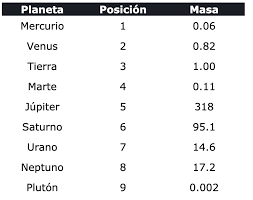
\includegraphics{figuras/tabla-ejemplo.png}\\
    {\textit{\small Fuente: } \textit{\small Autores por apellido (año). Titulo del documento de donde se copio la figura.}}
    \label{Tabla: Tabla ejemplo}
    \addcontentsline{lot}{table}{Tabla \arabic{cap1}.\arabic{tabla}: \descripcion}
    \addtocounter{tabla}{1}
\end{table}
% \label nos permite referenciar la tabla/figura en otra parte del documento.

% Subtitulo de ejemplo 1.1.1
\subsection{1.1.1 Subtitulo de ejemplo 1}

Lorem ipsum dolor sit amet, consectetur adipiscing elit, sed do eiusmod tempor incididunt ut labore et dolore magna aliqua. Ut enim ad minim veniam, quis nostrud exercitation ullamco laboris nisi ut aliquip ex ea commodo consequat. Duis aute irure dolor in reprehenderit in voluptate velit esse cillum dolore eu fugiat nulla pariatur. Excepteur sint occaecat cupidatat non proident, sunt in culpa qui officia deserunt mollit anim id est laborum.

% Subtitulo de ejemplo 1.1.2
\subsection{1.1.2 Subtitulo de ejemplo 2}

Lorem ipsum dolor sit amet, consectetur adipiscing elit, sed do eiusmod tempor incididunt ut labore et dolore magna aliqua. Ut enim ad minim veniam, quis nostrud exercitation ullamco laboris nisi ut aliquip ex ea commodo consequat. Duis aute irure dolor in reprehenderit in voluptate velit esse cillum dolore eu fugiat nulla pariatur. Excepteur sint occaecat cupidatat non proident, sunt in culpa qui officia deserunt mollit anim id est laborum.

% Subtitulo de ejemplo 1.1.3
\subsection{1.1.3 Subtitulo de ejemplo 3}

Lorem ipsum dolor sit amet, consectetur adipiscing elit, sed do eiusmod tempor incididunt ut labore et dolore magna aliqua. Ut enim ad minim veniam, quis nostrud exercitation ullamco laboris nisi ut aliquip ex ea commodo consequat. Duis aute irure dolor in reprehenderit in voluptate velit esse cillum dolore eu fugiat nulla pariatur. Excepteur sint occaecat cupidatat non proident, sunt in culpa qui officia deserunt mollit anim id est laborum.

%-------------------------------------------------------------------------
% Titulo de ejemplo 1.2
\section{1.2 Agregar formulas matemáticas}

Para agregar formulas matematicas en el texto se deben escribir entre "$ $", aquí podemos ver un ejemplo: 
El área de un círculo de radio r se puede calcular mediante la fórmula $A = \pi r^2$.
Fórmula para calcular la suma de los primeros n números enteros:  
\begin{equation}
    \sum_{i=1}^{n} i = \frac{n(n+1)}{2}
\end{equation}

Fórmula cuadrática:
\begin{equation}
    x = \frac{-b \pm \sqrt{b^2 - 4ac}}{2a}
\end{equation}

Teorema de Pitágoras:
\begin{equation}
    c = \sqrt{a^2 + b^2}
\end{equation}

Función exponencial:
\begin{equation}
    f(x) = e^x
\end{equation}

Fórmula de Euler:
\begin{equation}
    e^{i\theta} = \cos\theta + i\sin\theta
\end{equation}

Ley de Ohm:
\begin{equation}
    V = IR
\end{equation}


%-------------------------------------------------------------------------
% Titulo de ejemplo 1.3
\section{1.3 Titulo de ejemplo 3}

Lorem ipsum dolor sit amet, consectetur adipiscing elit, sed do eiusmod tempor incididunt ut labore et dolore magna aliqua. Ut enim ad minim veniam, quis nostrud exercitation ullamco laboris nisi ut aliquip ex ea commodo consequat. Duis aute irure dolor in reprehenderit in voluptate velit esse cillum dolore eu fugiat nulla pariatur. Excepteur sint occaecat cupidatat non proident, sunt in culpa qui officia deserunt mollit anim id est laborum.

% Modificar "\newcommand{\descripcion}{....} para describir el contenido de la tabla.
% Modificar la fuente según corresponda. 
% Puede ajustar el tamaño de la figura modificando el parametro "scale", ej: 0.5 (1 corresponde al tamaño original)
\begin{figure}[H]
    \centering
    \newcommand{\descripcion}{Descripción de la figura.}
    \caption*{Figura \arabic{cap1}.\arabic{figura}: \descripcion}
    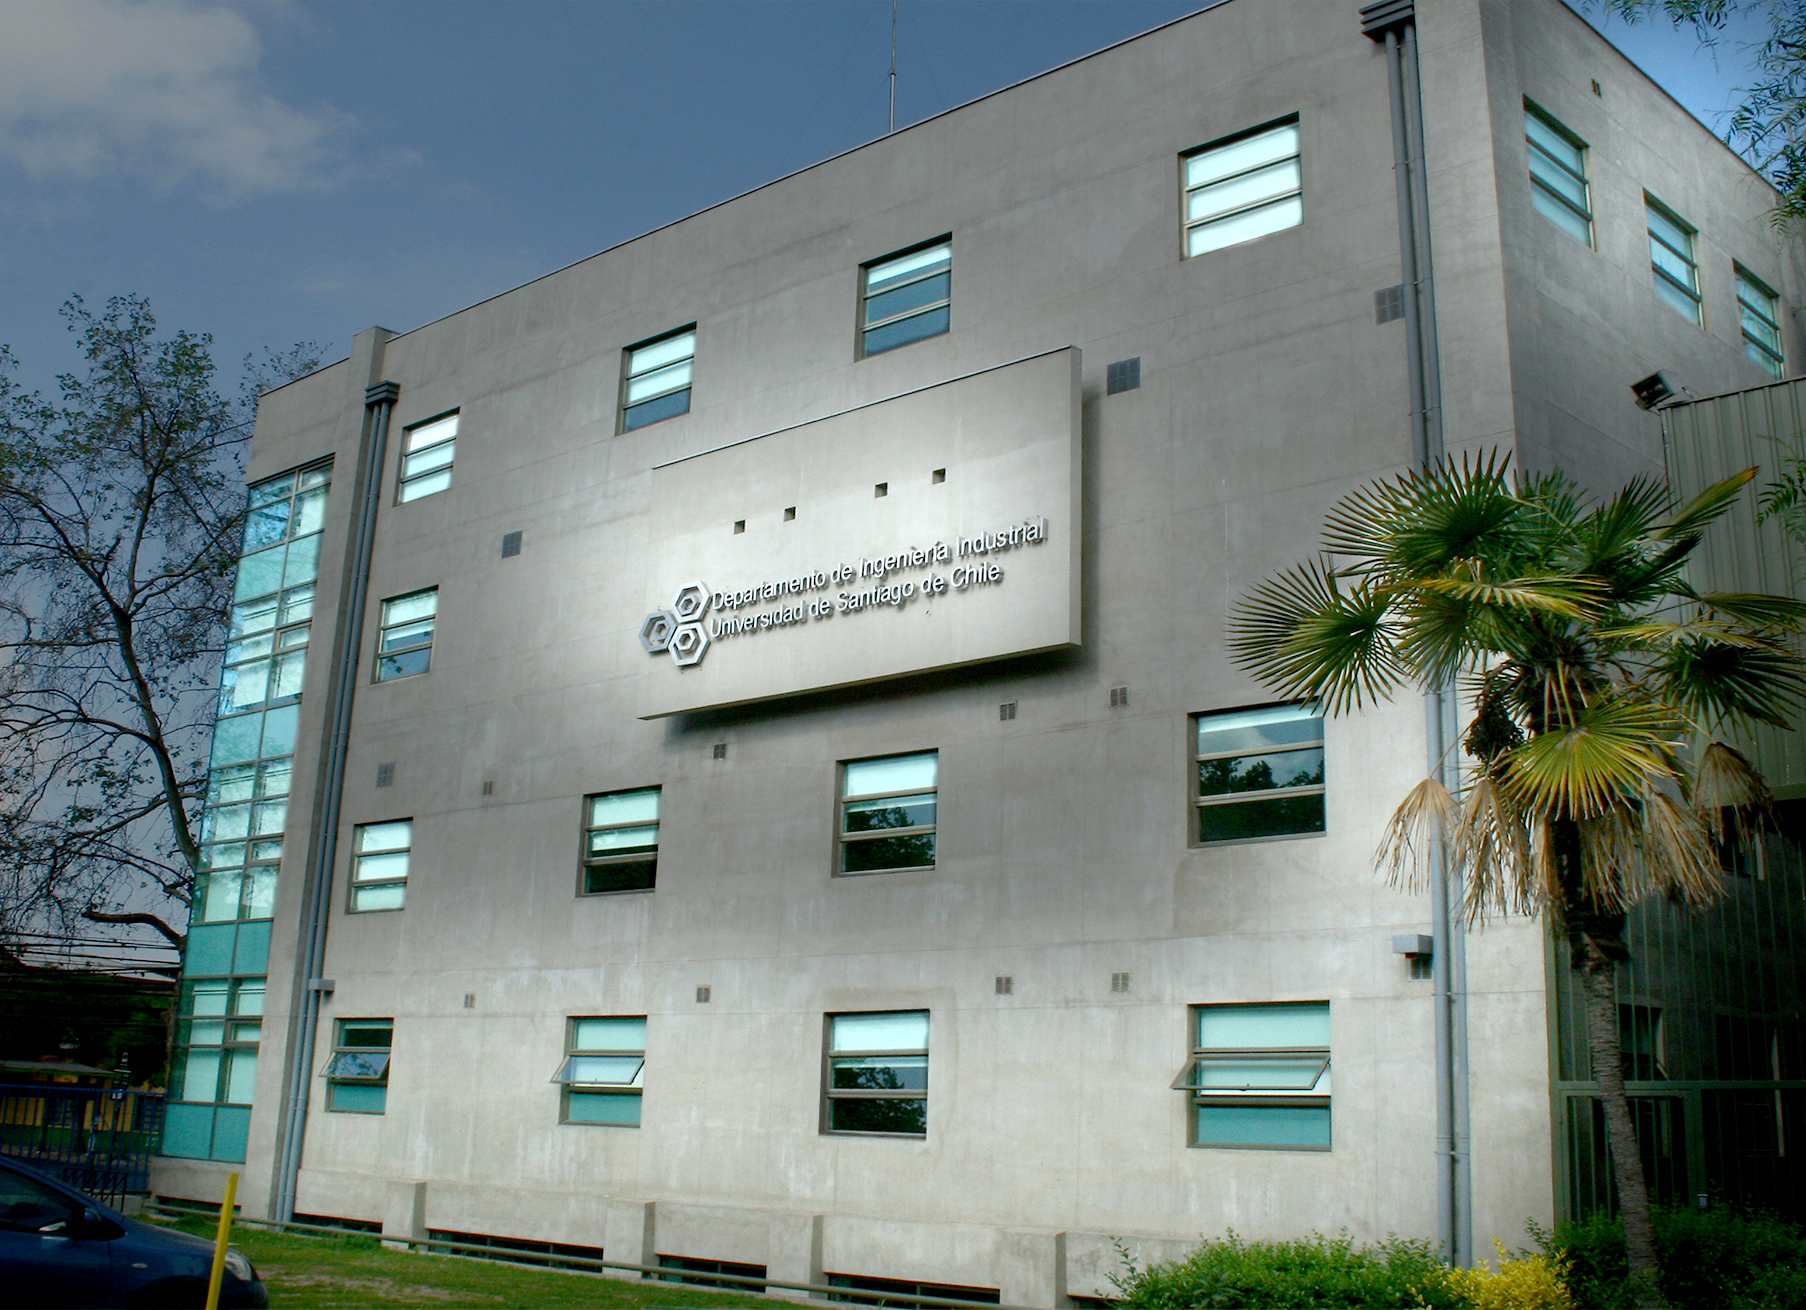
\includegraphics[scale=0.2]{figuras/dpto-industrias-usach.jpg}\\
    {\textit{\small Fuente: } \textit{\small Autores por apellido (año). Titulo del documento de donde se copio la figura.}}
    \label{fig:Dpto_Industrias}
    \addcontentsline{lof}{figure}{Figura \arabic{cap1}.\arabic{figura}: \descripcion}
    \addtocounter{figura}{1}
\end{figure}
% \label nos permite referenciar la tabla/figura en otra parte del documento.

%------------------------------------------------------------------------
% Titulo de ejemplo 1.4
\section{1.4 Listando información}

Para listar información se presentan 2 formas de hacerlo; de forma ordenada y de forma desordenada. A continuación se presenta en más detalle cada una de ellas

% Subtitulo de ejemplo 1.4.1
\subsection{1.4.1 Listar en forma ordenada}

A continuación un ejemplo de como listar información en forma ordenada:
\begin{enumerate}
    \item Ejemplo 1
    \item Ejemplo 2
    \item Ejemplo 3
    \item Ejemplo 4
\end{enumerate}

% Subtitulo de ejemplo 1.4.2
\subsection{1.4.2 Listar en forma desordenada}

A continuación un ejemplo de como listar información en forma desordenada:
\begin{itemize}
    \item Ejemplo 1
    \item Ejemplo 2
    \item Ejemplo 3
    \item Ejemplo 4
\end{itemize}
        \chapter*{CAPITULO II TITULO DEL CAPITULO}
\addcontentsline{toc}{chapter}{CAPITULO II TITULO DEL CAPITULO}
\setcounter{figura}{1}
\setcounter{tabla}{1}
%-------------------------------------------------------------------------
% Titulo de ejemplo 2.1
\section{2.1 Titulo de ejemplo 1}

% Modificar "\newcommand{\descripcion}{....} para describir el contenido de la tabla.
% Modificar la fuente según corresponda. 
\begin{table}[H]
    \centering
    \newcommand{\descripcion}{Descripción de la tabla.}
    \caption*{Tabla \arabic{cap2}.\arabic{tabla}: \descripcion}
    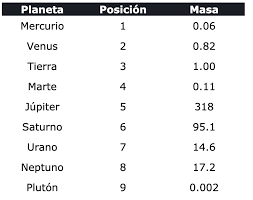
\includegraphics{figuras/tabla-ejemplo.png}\\
    {\textit{\small Fuente: } \textit{\small Autores por apellido (año). Titulo del documento de donde se copio la figura.}}
    \label{Tabla: Tabla ejemplo 2}
    \addcontentsline{lot}{table}{Tabla \arabic{cap2}.\arabic{tabla}: \descripcion}
    \addtocounter{tabla}{1}
\end{table}
% \label nos permite referenciar la tabla/figura en otra parte del documento.

Lorem ipsum dolor sit amet, consectetur adipiscing elit, sed do eiusmod tempor incididunt ut labore et dolore magna aliqua. Ut enim ad minim veniam, quis nostrud exercitation ullamco laboris nisi ut aliquip ex ea commodo consequat. Duis aute irure dolor in reprehenderit in voluptate velit esse cillum dolore eu fugiat nulla pariatur. Excepteur sint occaecat cupidatat non proident, sunt in culpa qui officia deserunt mollit anim id est laborum.
%-------------------------------------------------------------------------
% Titulo de ejemplo 2.2
\section{2.2 Titulo de ejemplo 2}
Lorem ipsum dolor sit amet, consectetur adipiscing elit, sed do eiusmod tempor incididunt ut labore et dolore magna aliqua. Ut enim ad minim veniam, quis nostrud exercitation ullamco laboris nisi ut aliquip ex ea commodo consequat. Duis aute irure dolor in reprehenderit in voluptate velit esse cillum dolore eu fugiat nulla pariatur. Excepteur sint occaecat cupidatat non proident, sunt in culpa qui officia deserunt mollit anim id est laborum.

% Modificar "\newcommand{\descripcion}{....} para describir el contenido de la tabla.
% Modificar la fuente según corresponda. 
\begin{table}[H]
    \centering
    \newcommand{\descripcion}{Descripción de la tabla.}
    \caption*{Tabla \arabic{cap2}.\arabic{tabla}: \descripcion}
    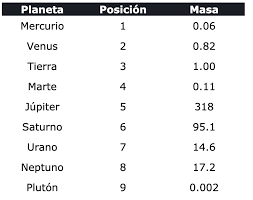
\includegraphics{figuras/tabla-ejemplo.png}\\
    {\textit{\small Fuente: } \textit{\small Autores por apellido (año). Titulo del documento de donde se copio la figura.}}
    \label{Tabla: Tabla ejemplo 3}
    \addcontentsline{lot}{table}{Tabla \arabic{cap2}.\arabic{tabla}: \descripcion}
    \addtocounter{tabla}{1}
\end{table}
% \label nos permite referenciar la tabla/figura en otra parte del documento.

%-------------------------------------------------------------------------
% Titulo de ejemplo 2.3
\section{2.3 Titulo de ejemplo 3}
Para escribir palabras y sus definiciones con una sangría después de los dos puntos, puedes utilizar el entorno de lista 'description' de LaTeX.

Puedes ajustar el espaciado entre la deinifición y los 2 puntos, y la sangría según tus preferencias utilizando los comandos labelwidth y leftmargin dentro del entorno description.
Por ejemplo:

\begin{description}[labelwidth=1.2cm, leftmargin=1.5cm]
\item[ESIG]: Encargado del sistema integrado de gestión plantas de alimentos Agrosuper.
\item[EPS]: Encargado del sistema integrado de gestión Planta.
\item[HACCP]: Siglas en inglés Hazard Analysis \& Critical Control Points, que significan Análisis de Peligros y Puntos Críticos de Control.
\item[MSIG]: Manual del Sistema Integrado de Gestión.
\item[R\&A]: Responsabilidad y autoridad.
\item[SGA]: Sistema de Gestión Ambiental basado en la norma ISO 14001:2015.
\item[SGS]: Sistema de Gestión de Salud y Seguridad Ocupacional basado en la norma ISO 
 45001: 2018.
\item[SGC]: Sistema de Gestión de Calidad basado en la norma ISO 9001:2015.
\item[SGIA]: Sistema de gestión de la inocuidad de los alimentos basado en la norma ISO 
 22000:2018.
\item[PPR]: Programa de prerrequisitos.
\item[PPRO]: Programa de prerrequisitos Operativos.
\item[SIG]: Sistema Integrado de Gestión, conformado por las normas ISO 9001:2015, ISO 
 14001:2015, ISO 45001:2018 e ISO 22000:2018.
\item[PDI]: “Pellets Durability Index” en inglés, acrónimo para determinar dureza del alimento, esta debe resistir íntegramente hasta el comedero del ave. 
\item[OPA]: “Optimización de Proceso Animal” Buscar de manera organizada y sistematizada 
 un animal óptimo para la rentabilidad del negocio.
\end{description}

En este ejemplo, el ancho del espacio para los términos se ha establecido en 1.2cm (labelwidth) y la sangría se ha establecido en 1.5cm (leftmargin). Puedes ajustar estos valores según tus necesidades.

\textbf{Lo mismo que antes, pero poniendo los 2 puntos dentro de los corchetes (no son considerados en el espaciado). Puede elegir la opción que más prefiera.}

\begin{description}[labelwidth=1.3cm, leftmargin=1.5cm]
\item[ESIG:] Encargado del sistema integrado de gestión plantas de alimentos Agrosuper.
\item[EPS:] Encargado del sistema integrado de gestión Planta.
\item[HACCP:] Siglas en inglés Hazard Analysis \& Critical Control Points, que significan Análisis de Peligros y Puntos Críticos de Control.
\item[MSIG:] Manual del Sistema Integrado de Gestión.
\item[R\&A:] Responsabilidad y autoridad.
\item[SGA:] Sistema de Gestión Ambiental basado en la norma ISO 14001:2015.
\item[SGS:] Sistema de Gestión de Salud y Seguridad Ocupacional basado en la norma ISO 
 45001: 2018.
\item[SGC:] Sistema de Gestión de Calidad basado en la norma ISO 9001:2015.
\item[SGIA:] Sistema de gestión de la inocuidad de los alimentos basado en la norma ISO 
 22000:2018.
\item[PPR] Programa de prerrequisitos.
\item[PPRO:] Programa de prerrequisitos Operativos.
\item[SIG:] Sistema Integrado de Gestión, conformado por las normas ISO 9001:2015, ISO 
 14001:2015, ISO 45001:2018 e ISO 22000:2018.
\item[PDI:] “Pellets Durability Index” en inglés, acrónimo para determinar dureza del alimento, esta debe resistir íntegramente hasta el comedero del ave. 
\item[OPA:] “Optimización de Proceso Animal” Buscar de manera organizada y sistematizada 
 un animal óptimo para la rentabilidad del negocio.
\end{description}

\textbf{SI DESEA ESCRIBIR EN EL TEXTO UN AMPERSAND (\&) DEBE HACERLO PONIENDO UN BACKSLASH (\textbackslash) ANTES DEL AMPERSAND, YA QUE SON CONSIDERADOS CARACTERES DE TABULACIÓN DE ALINEACIÓN EN LATEX. AL IGUAL QUE SI QUISIERA PONER UN PORCENTAJE (\%), YA QUE ESTOS SE UTILIZAN PARA HACER COMENTARIOS}
        \chapter*{CAPITULO III TITULO DEL CAPITULO}
\addcontentsline{toc}{chapter}{CAPITULO III TITULO DEL CAPITULO}
\setcounter{figura}{1}
\setcounter{tabla}{1}
%-------------------------------------------------------------------------
% Titulo de ejemplo 3.1
\section{3.1 Titulo de ejemplo 1}
Lorem ipsum dolor sit amet, consectetur adipiscing elit, sed do eiusmod tempor incididunt ut labore et dolore magna aliqua. Ut enim ad minim veniam, quis nostrud exercitation ullamco laboris nisi ut aliquip ex ea commodo consequat. Duis aute irure dolor in reprehenderit in voluptate velit esse cillum dolore eu fugiat nulla pariatur. Excepteur sint occaecat cupidatat non proident, sunt in culpa qui officia deserunt mollit anim id est laborum.

% Modificar "\newcommand{\descripcion}{....} para describir el contenido de la tabla.
% Modificar la fuente según corresponda. 
% Puede ajustar el tamaño de la figura modificando el parametro "scale", ej: 0.5 (1 corresponde al tamaño original)
\begin{figure}[H]
    \centering
    \newcommand{\descripcion}{Descripción de la figura.}
    \caption*{Figura \arabic{cap3}.\arabic{figura}: \descripcion}
    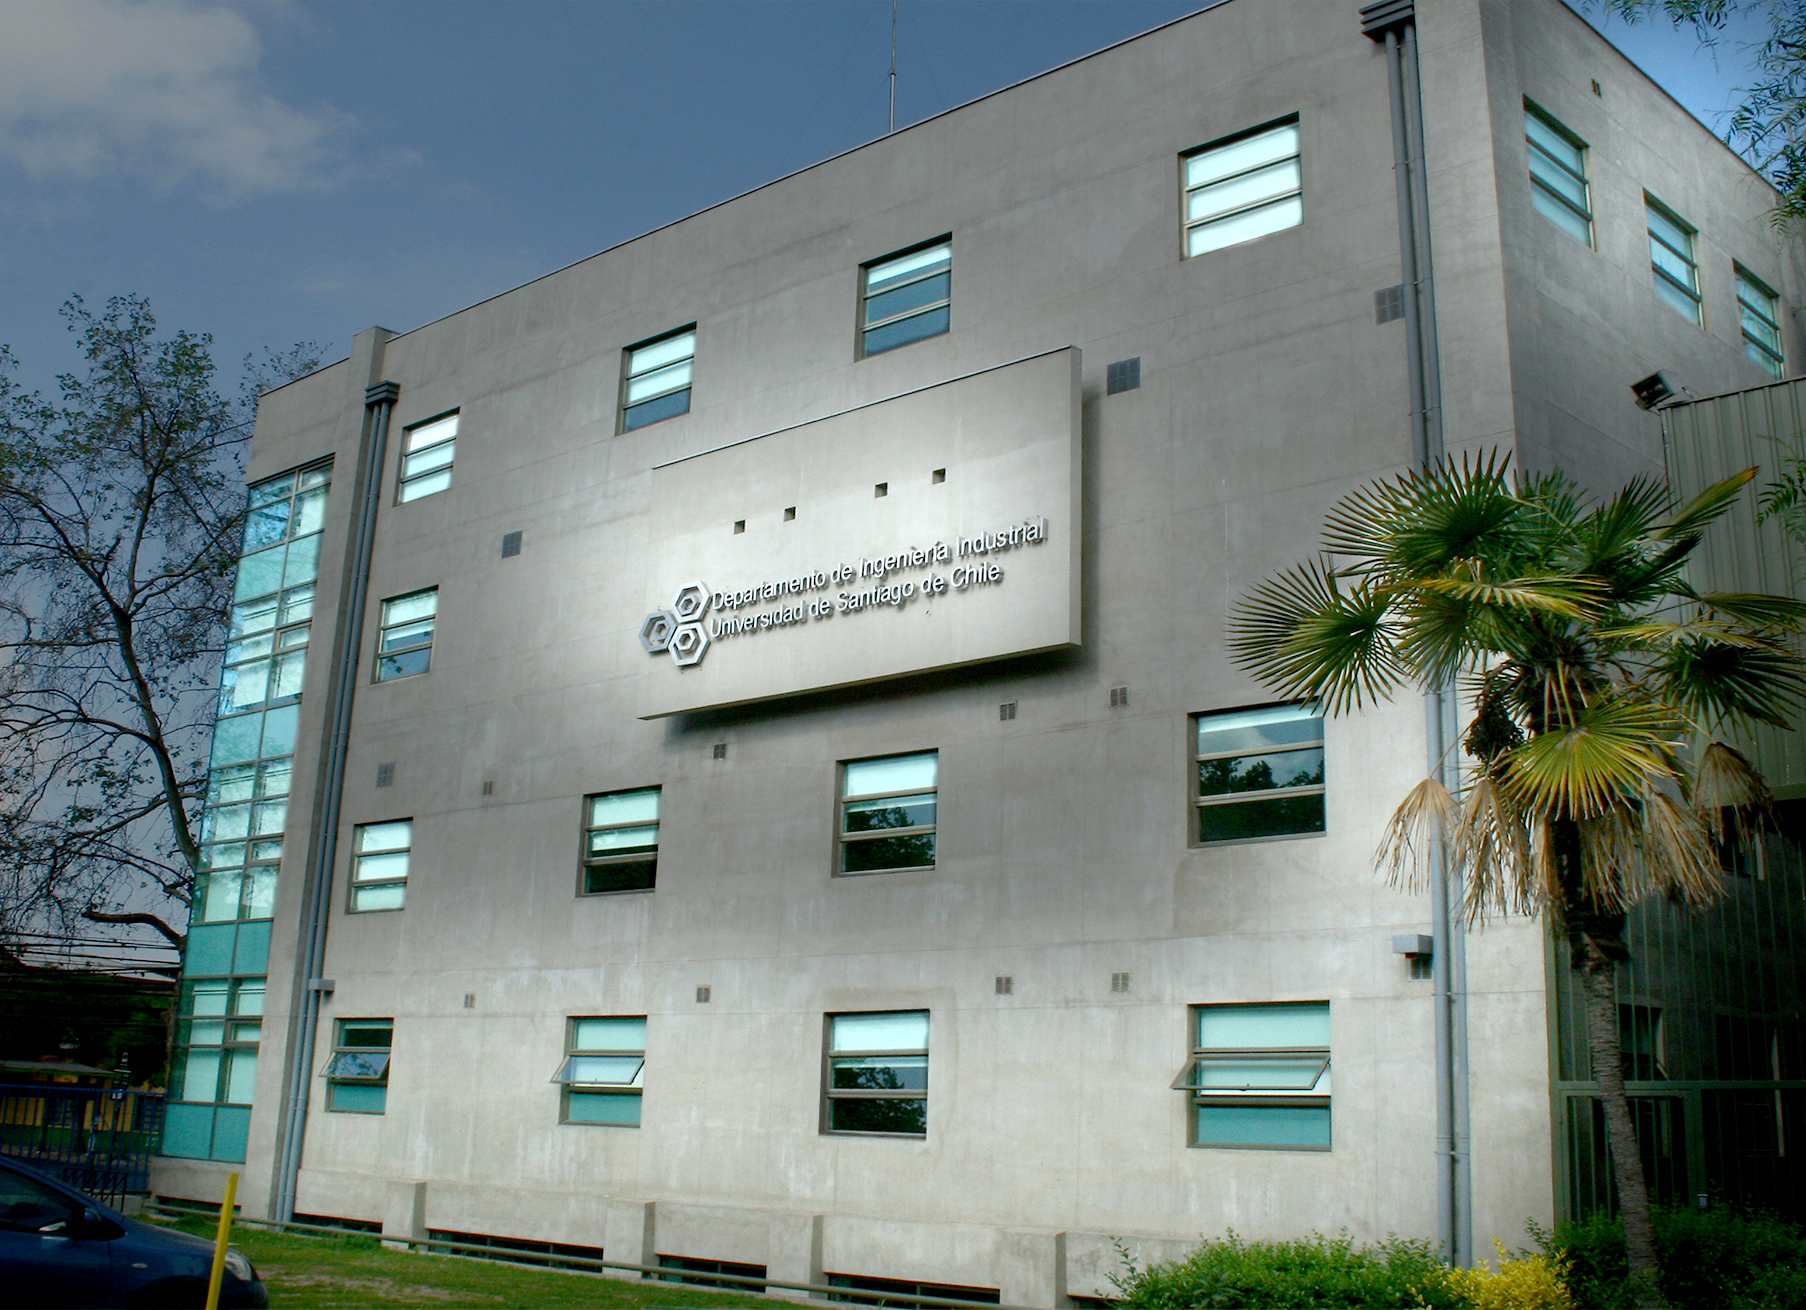
\includegraphics[scale=0.2]{figuras/dpto-industrias-usach.jpg}\\
    {\textit{\small Fuente: } \textit{\small Autores por apellido (año). Titulo del documento de donde se copio la figura.}}
    \label{fig:Dpto. Industrias 2}
    \addcontentsline{lof}{figure}{Figura \arabic{cap3}.\arabic{figura}: \descripcion}
    \addtocounter{figura}{1}
\end{figure}
% \label nos permite referenciar la tabla/figura en otra parte del documento.

%-------------------------------------------------------------------------
% Titulo de ejemplo 3.2
\section{3.2 Titulo de ejemplo 2}

% Modificar "\newcommand{\descripcion}{....} para describir el contenido de la tabla.
% Modificar la fuente según corresponda. 
% Puede ajustar el tamaño de la figura modificando el parametro "scale", ej: 0.5 (1 corresponde al tamaño original)
\begin{figure}[H]
    \centering
    \newcommand{\descripcion}{Descripción de la figura.}
    \caption*{Figura \arabic{cap3}.\arabic{figura}: \descripcion}
    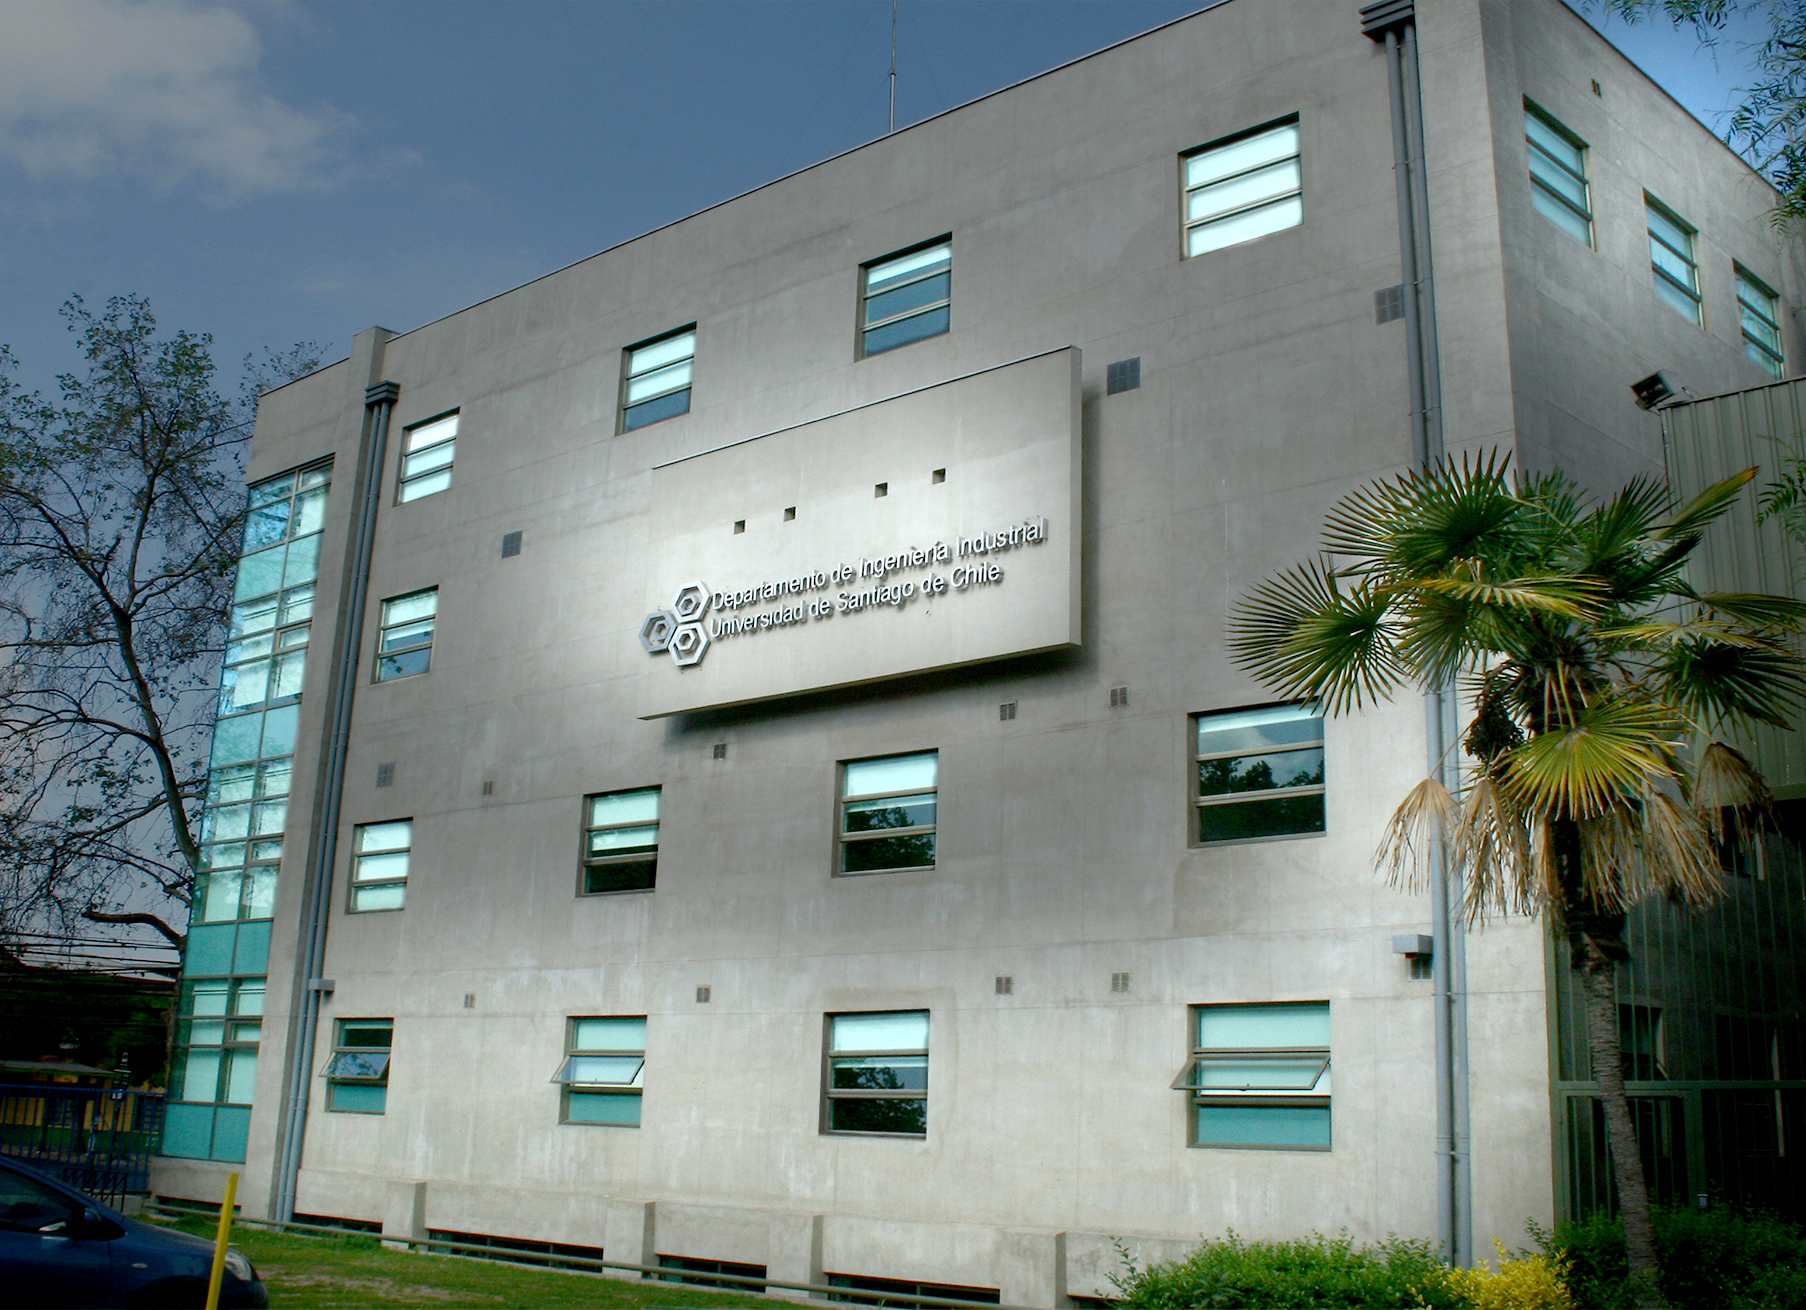
\includegraphics[scale=0.2]{figuras/dpto-industrias-usach.jpg}\\
    {\textit{\small Fuente: } \textit{\small Autores por apellido (año). Titulo del documento de donde se copio la figura.}}
    \label{fig:Dpto. Industrias 3}
    \addcontentsline{lof}{figure}{Figura \arabic{cap3}.\arabic{figura}: \descripcion}
    \addtocounter{figura}{1}
\end{figure}
% \label nos permite referenciar la tabla/figura en otra parte del documento.

Lorem ipsum dolor sit amet, consectetur adipiscing elit, sed do eiusmod tempor incididunt ut labore et dolore magna aliqua. Ut enim ad minim veniam, quis nostrud exercitation ullamco laboris nisi ut aliquip ex ea commodo consequat. Duis aute irure dolor in reprehenderit in voluptate velit esse cillum dolore eu fugiat nulla pariatur. Excepteur sint occaecat cupidatat non proident, sunt in culpa qui officia deserunt mollit anim id est laborum

%-------------------------------------------------------------------------
% Titulo de ejemplo 3.3
\section{3.3 Titulo de ejemplo 3}

Lorem ipsum dolor sit amet, consectetur adipiscing elit, sed do eiusmod tempor incididunt ut labore et dolore magna aliqua. Ut enim ad minim veniam, quis nostrud exercitation ullamco laboris nisi ut aliquip ex ea commodo consequat. Duis aute irure dolor in reprehenderit in voluptate velit esse cillum dolore eu fugiat nulla pariatur. Excepteur sint occaecat cupidatat non proident, sunt in culpa qui officia deserunt mollit anim id est laborum.

% Modificar "\newcommand{\descripcion}{....} para describir el contenido de la tabla.
% Modificar la fuente según corresponda. 
% Puede ajustar el tamaño de la figura modificando el parametro "scale", ej: 0.5 (1 corresponde al tamaño original)
\begin{figure}[H]
    \centering
    \newcommand{\descripcion}{Descripción de la figura.}
    \caption*{Figura \arabic{cap3}.\arabic{figura}: \descripcion}
    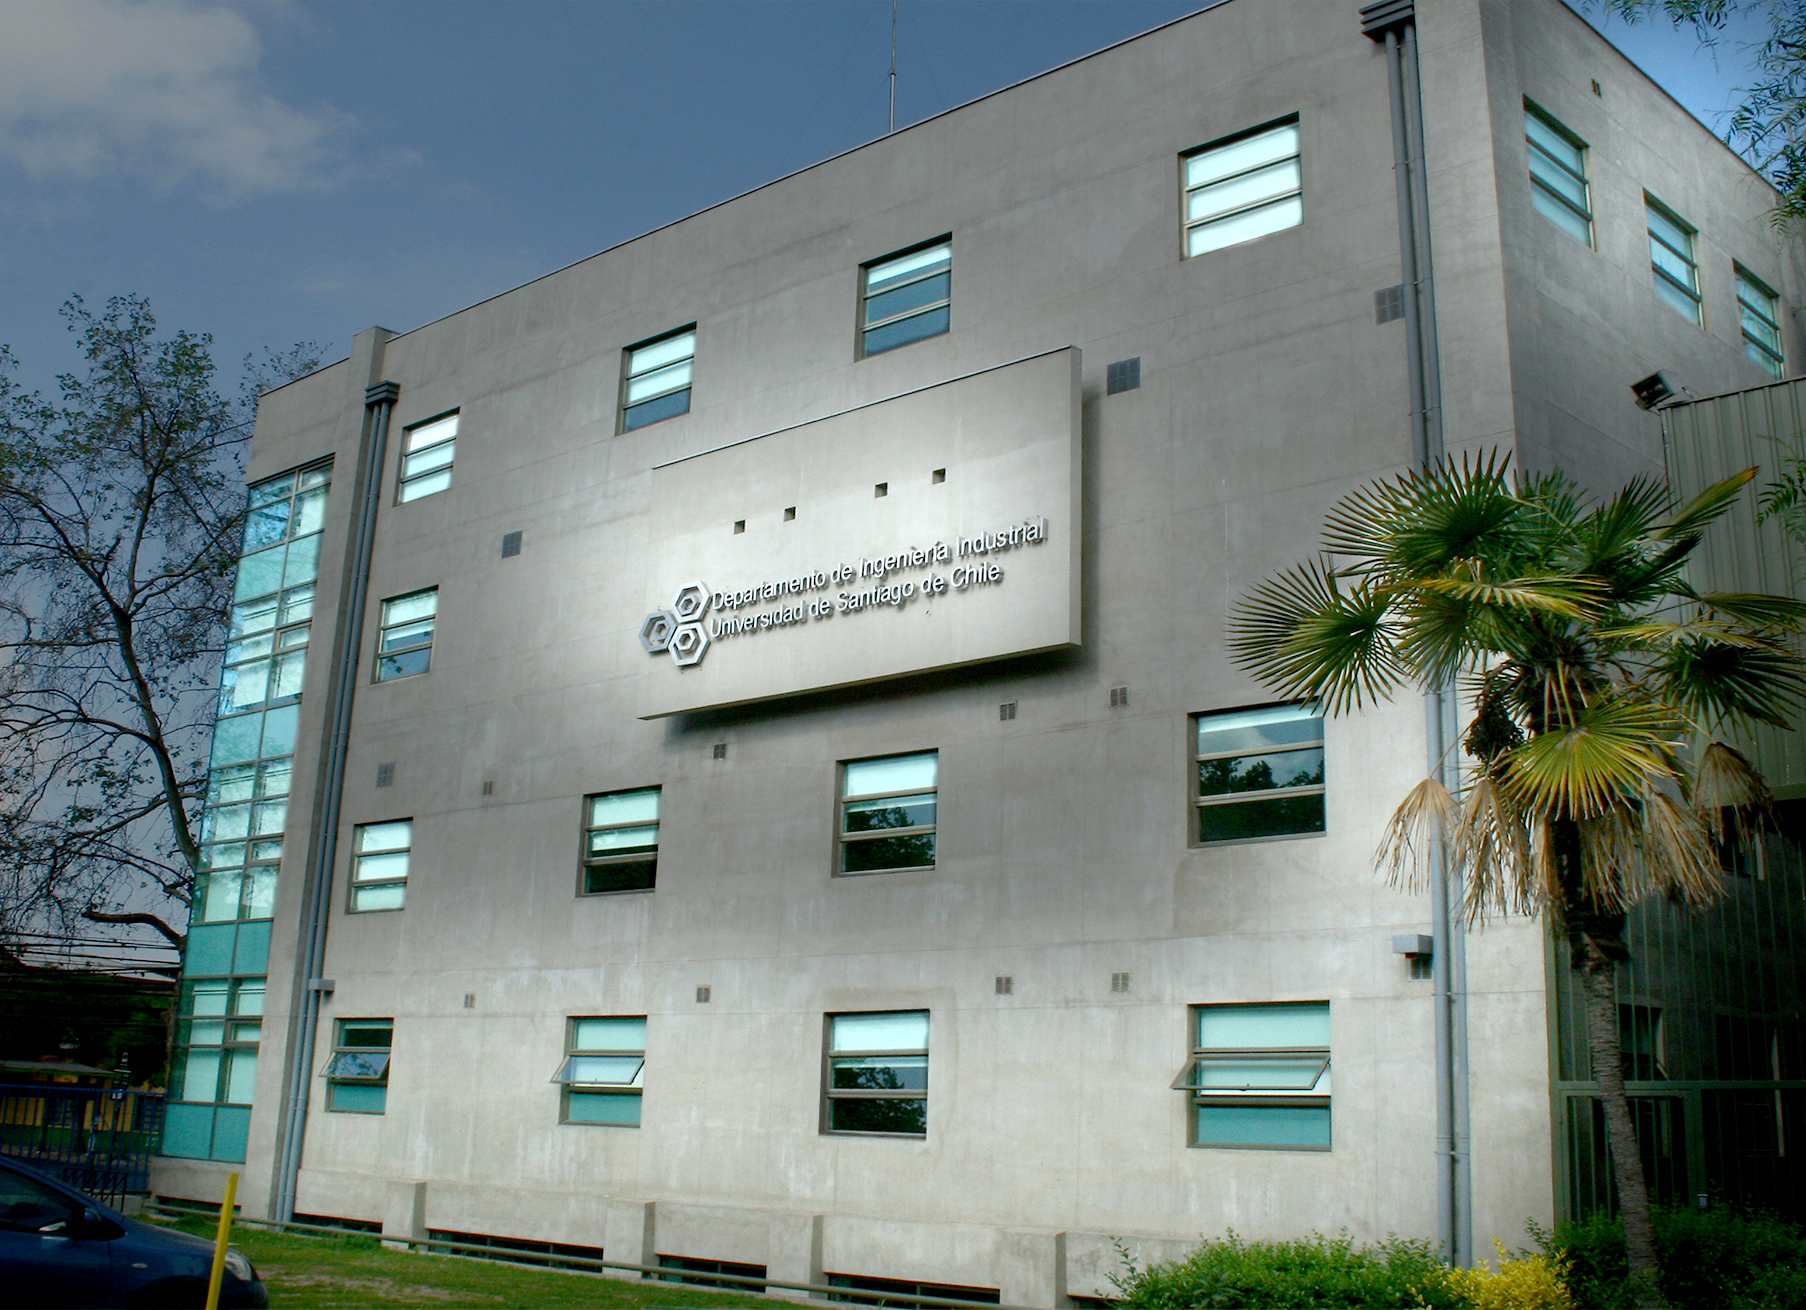
\includegraphics[scale=0.2]{figuras/dpto-industrias-usach.jpg}\\
    {\textit{\small Fuente: } \textit{\small Autores por apellido (año). Titulo del documento de donde se copio la figura.}}
    \label{fig:Dpto. Industrias 4}
    \addcontentsline{lof}{figure}{Figura \arabic{cap3}.\arabic{figura}: \descripcion}
    \addtocounter{figura}{1}
\end{figure}
% \label nos permite referenciar la tabla/figura en otra parte del documento.

En el caso de querer listar información de algún tipo, es posible hacerlo con 
        \chapter*{CAPITULO IV TITULO DEL CAPITULO}
\addcontentsline{toc}{chapter}{CAPITULO IV TITULO DEL CAPITULO}
%-------------------------------------------------------------------------
En este capítulo se pretende profundizar en las citas, por lo que se presentará una gran variedad de ejemplos para hacerlos dependiendo del tipo de cita deseado.

% Titulo de ejemplo 4.1
\section{4.1 Referencias en APA}

\subsection{4.1.1 Cita como mención del/los autor(es)}

% Cita en mención de un autor
\subsection*{Mencionando un autor}

Contenido de ejemplo según \textcite{articulo:ejemplo_2}, que explica las diferentes formas de citar en Latex.


%Cita en mención de varios autores
\subsection*{Mencionando varios autores}

Contenido de ejemplo según \textcite{libro:ejemplo_varios_autores}, que explica las diferentes formas de citar en Latex.


\subsection{4.1.2 Citando al final del parrafo o idea}

\subsection*{Citando un autor}

Lorem ipsum dolor sit amet, consectetur adipiscing elit, sed do eiusmod tempor incididunt ut labore et dolore magna aliqua. Ut enim ad minim veniam, quis nostrud exercitation ullamco laboris nisi ut aliquip ex ea commodo consequat \parencite{articulo:ejemplo_2}.


\subsection*{Citando varios autores}

Lorem ipsum dolor sit amet, consectetur adipiscing elit, sed do eiusmod tempor incididunt ut labore et dolore magna aliqua. Ut enim ad minim veniam, quis nostrud exercitation ullamco laboris nisi ut aliquip ex ea commodo consequat \parencite{libro:ejemplo_varios_autores}.


\subsection*{Citando a más de 3 autores}
En este caso se presentará cuando se quiere referir al autor a mitad del texto, por ejemplo cuando se dice: según \textcite{articulo:ejemplo_1} dice que \textit{"Podremos citar de muchas maneras diferentes en Latex, y podemos obtener más información en la documentación de Overleaf: https://es.overleaf.com/learn"} o también cuando queremos hacer la cita al final del texto como en este caso \parencite{articulo:ejemplo_1}.


\subsection{4.1.3 Citando con número de pagina}

Para citar con numeros de pagina puede utilizar los mismos comandos explicados en los subcapitulos anteriores, por ejemplo, según \textcite[p. 7]{libro:ejemplo_2}, que explica las diferentes formas de citar en Latex.

Si queremos citar con un intevalo de paginas podemos hacerlo con solo escribir el intervalo antre guion, como lo menciona \textcite[p. 32-39]{articulo:ejemplo_1}. También podemos hacerlo con 'parencite', como se ve a continuación \parencite[p. 32-39]{articulo:ejemplo_1}.

En el caso que los números de páginas que se desea referenciar no son correlativos, sino diferentes, se hace tan solo separandolos con una coma, como se ve a continuación \parencite[p. 23, 37, 39]{articulo:ejemplo_1}.

Agregamos algunas citas para tenerlas de ejemplo, ya que, según \textcite{Gorman2020} es una buena forma de comprender mejor las cosas. Al final de este parrafo agregaremos una ultima cita para terminar \parencite{Garcia2019}
%-------------------------------------------------------------------------
        \chapter*{CAPITULO V TITULO DEL CAPITULO}
\addcontentsline{toc}{chapter}{CAPITULO V TITULO DEL CAPITULO}
%-------------------------------------------------------------------------
% Titulo de ejemplo 5.1
\section{5.1 Titulo de ejemplo 1}

Lorem ipsum dolor sit amet, consectetur adipiscing elit, sed do eiusmod tempor incididunt ut labore et dolore magna aliqua. Ut enim ad minim veniam, quis nostrud exercitation ullamco laboris nisi ut aliquip ex ea commodo consequat. Duis aute irure dolor in reprehenderit in voluptate velit esse cillum dolore eu fugiat nulla pariatur. Excepteur sint occaecat cupidatat non proident, sunt in culpa qui officia deserunt mollit anim id est laborum.
%-------------------------------------------------------------------------
% Titulo de ejemplo 5.2
\section{5.2 Titulo de ejemplo 2}

Lorem ipsum dolor sit amet, consectetur adipiscing elit, sed do eiusmod tempor incididunt ut labore et dolore magna aliqua. Ut enim ad minim veniam, quis nostrud exercitation ullamco laboris nisi ut aliquip ex ea commodo consequat. Duis aute irure dolor in reprehenderit in voluptate velit esse cillum dolore eu fugiat nulla pariatur. Excepteur sint occaecat cupidatat non proident, sunt in culpa qui officia deserunt mollit anim id est laborum.
%-------------------------------------------------------------------------
% Titulo de ejemplo 5.3
\section{5.3 Titulo de ejemplo 3}

Lorem ipsum dolor sit amet, consectetur adipiscing elit, sed do eiusmod tempor incididunt ut labore et dolore magna aliqua. Ut enim ad minim veniam, quis nostrud exercitation ullamco laboris nisi ut aliquip ex ea commodo consequat. Duis aute irure dolor in reprehenderit in voluptate velit esse cillum dolore eu fugiat nulla pariatur. Excepteur sint occaecat cupidatat non proident, sunt in culpa qui officia deserunt mollit anim id est laborum.
        \chapter*{CAPITULO VI CONCLUSIONES}
\addcontentsline{toc}{chapter}{CONCLUSIONES}

Lorem ipsum dolor sit amet, consectetur adipiscing elit, sed do eiusmod tempor incididunt ut labore et dolore magna aliqua. Ut enim ad minim veniam, quis nostrud exercitation ullamco laboris nisi ut aliquip ex ea commodo consequat. Duis aute irure dolor in reprehenderit in voluptate velit esse cillum dolore eu fugiat nulla pariatur. Excepteur sint occaecat cupidatat non proident, sunt in culpa qui officia deserunt mollit anim id est laborum.

Lorem ipsum dolor sit amet, consectetur adipiscing elit, sed do eiusmod tempor incididunt ut labore et dolore magna aliqua. Ut enim ad minim veniam, quis nostrud exercitation ullamco laboris nisi ut aliquip ex ea commodo consequat. Duis aute irure dolor in reprehenderit in voluptate velit esse cillum dolore eu fugiat nulla pariatur. Excepteur sint occaecat cupidatat non proident, sunt in culpa qui officia deserunt mollit anim id est laborum.

Lorem ipsum dolor sit amet, consectetur adipiscing elit, sed do eiusmod tempor incididunt ut labore et dolore magna aliqua. Ut enim ad minim veniam, quis nostrud exercitation ullamco laboris nisi ut aliquip ex ea commodo consequat. Duis aute irure dolor in reprehenderit in voluptate velit esse cillum dolore eu fugiat nulla pariatur. Excepteur sint occaecat cupidatat non proident, sunt in culpa qui officia deserunt mollit anim id est laborum.

Lorem ipsum dolor sit amet, consectetur adipiscing elit, sed do eiusmod tempor incididunt ut labore et dolore magna aliqua. Ut enim ad minim veniam, quis nostrud exercitation ullamco laboris nisi ut aliquip ex ea commodo consequat. Duis aute irure dolor in reprehenderit in voluptate velit esse cillum dolore eu fugiat nulla pariatur. Excepteur sint occaecat cupidatat non proident, sunt in culpa qui officia deserunt mollit anim id est laborum.
        
    {
        \backmatter
        \printbibliography
    }

    \appendix
    \begin{appendices}
        \chapter*{ANEXOS}
\addcontentsline{toc}{chapter}{ANEXOS}
    \end{appendices}
    % \clearpage
    % \addappheadtotoc
    % \appendixpage
\end{document}


%-----------------------------------------------------------------------------------------------------------------------------------------